% TODO Matthias: Switch font size to 12 pt
\documentclass[11pt, oneside]{article}

\usepackage[utf8]{inputenc}

\title{An Investigation into Environmental Sustainability COMP90024 - Team 24}


\author{Matthias Bachfischer\thanks{\tt \space Student ID: 1133751 - m.bachfischer@student.unimelb.edu.au } \qquad Parikshit Diwan \thanks{\tt  \space Student ID: 1110497 - pdiwan@student.unimelb.edu.au } \\ \\
\qquad Liam Simon \thanks{\tt  \space Student ID: 1128453 - ljsimon@student.unimelb.edu.au } \qquad Rejoy Benjamin \thanks{\tt  \space Student ID: 1110935 - rbenjamin@student.unimelb.edu.au } \\ \\
\qquad Colin McLean \thanks{\tt  \space Student ID: 1139518 - cmmclea@student.unimelb.edu.au }
\\ \\ \\
   COMP90024 Cluster and Cloud Computing \\ \\
     The University of Melbourne \\
}
\date{\today}

% Import references from Endnote
\usepackage[backend=biber,style=apa,natbib=true]{biblatex}
\DeclareLanguageMapping{english}{english-apa}
\addbibresource{references.bib}

% Define acronyms - use \acrfull and \acrshort to use acronyms
\usepackage[acronym]{glossaries}

% Insert acronyms
\newacronym{api}{API}{Application Programming Interface}
\newacronym{aurin}{AURIN}{Australian Urban Research Infrastructure Network}
\newacronym{cer}{CER}{Clean Energy Regulator}
\newacronym{gccsa}{GCCSA}{Greater Capital City Statistical Areas}
\newacronym{iaac}{IaaC}{Infrastructure as Code}
\newacronym{json}{JSON}{JavaScript Object Notation}
\newacronym{ncris}{NCRIS}{National Collaborative Research Infrastructure Strategy}
\newacronym{rest}{REST}{Representational State Transfer}
\newacronym{tcp}{TCP}{Transmission Control Protocol}
\newacronym{url}{URL}{Uniform Resource Locator}
\newacronym{uuid}{UUID}{Universally unique identifier}

% Enable table formatting
\usepackage{graphicx}
\usepackage{subcaption}
\usepackage[export]{adjustbox}

% Configure continuous counting of figures and tables across sections
\usepackage{chngcntr}
\counterwithout{figure}{section}
\counterwithout{table}{section}

% Wrap figures with the text
\usepackage{wrapfig}

% Smaller fontsize for footnotes
\usepackage{hyperref}
\usepackage{relsize}


\renewcommand*{\UrlFont}{\ttfamily\smaller\relax}  
 
% Easy quotes
\usepackage{csquotes}

% Create TODOs
\usepackage[colorinlistoftodos,prependcaption]{todonotes}

% reduce spacing in enumeration
\newenvironment{myitemize}
{ \begin{itemize}
    \setlength{\itemsep}{1pt}
    \setlength{\parskip}{1pt}
    \setlength{\parsep}{1pt}     }
{ \end{itemize}                  } 

\begin{document}

\maketitle

\begin{abstract}
In this report, the system and application architecture that was implemented for assignment 2 of the COMP90024 Cluster and Cloud Computing course at the University of Melbourne is presented. The scenario that was chosen for this assignment is related to the topic of environmental sustainability and how it can be linked to user activity in online social media networks such as Twitter. 
\newline
The report at hand includes an in-depth discussion of each individual system component that is part of the architecture and also outlines the collaboration within the team during the implementation of the system.
\newline 
The accompanying source code for this assignment is publicly available and can be found under the following Git repository \acrshort{url}:
\newline
\url{https://github.com/Bachfischer/cluster-and-cloud-computing-assignment-2}.
\end{abstract}

\newpage

\tableofcontents

\newpage

\section{Introduction}
The topic of environmental sustainability has gained significant momentum within the public discourse over the recent years with various environmental organizations such as Greenpeace or the World Resource Institute which have long been advocating for a more sustainable way of living. Over the last 5+ years, new movements such as \enquote{Fridays for Future} protests have emerged and gained a lot of attention in the news and media. Given the increasing importance of online social media networks such as Twitter, it is not surprising that a tremendous amount of the discussions and sharing of information has also occurred in such networks. 
\newline
\newline
The objective of the scenario that was chosen for this assignment was to analyze the Twitter activity of the geographic region of Australia with respect to environmental sustainability. In particular, the focus of the scenario was to analyze whether the amount of online social media activity on Twitter in a particular region correlates with the number of solar panel installations in that region. 
\newline
By comparing the amount of tweet activity with the number of solar panel installations, the authors of this paper wanted to evaluate whether people really choose to  \enquote{put their money where their mouth is} when it comes to protecting the environment and living a more sustainable life. Section \ref{sec:scenario_description_environmental_sustainability} provides further context about this scenario.
\newline
\newline
The general system architecture as well as the deployment of the various components on the University of Melbourne Research Cloud is described in section \ref{sec:system_architecture}. The system architecture is designed for operation in a cloud environment - it is highly scalable and can be fully orchestrated via the Ansible scripting technology \citep{ansible}. Docker \citep{docker} is used to manage and deploy application components across the four computing nodes that were allocated by the course instructors to the project team. Section \ref{sec:cloud_infrastructure} describes in detail how those technologies were leveraged for the assignment.
\newline
\newline
For the study, a large Twitter dataset consisting of tweets from five different cities across Australia (Sydney, Melbourne, Adelaide, Perth and Canberra) was collected. The dataset was extracted from Twitter based on static keyword filtering and exclusively contains tweets that mention the topic of environmental sustainability. Further implementation notes on the architecture of the Twitter data harvesting system can be found in section \ref{sec:data_collection}. 
\newline
\newline
The system makes use of the CouchDB database technology \citep{couchdb} to provide storage and persistence functionality. The CouchDB setup and the most relevant databases are further described in section \ref{sec:data_storage}
\newline
\newline
For comparison of the collected tweet data with statistical data from the \acrfull{aurin}, the \acrfull{cer} dataset was used. Various processing steps, e.g. conversion of GPS coordinates to postcodes as well as MapReduce-based analytics had to be applied in order to process both the collected tweet data as well as the \acrshort{cer} dataset. These processing and analytics steps are further presented in section \ref{sec:data_processing}.
\newline
\newline
Users of the system have the ability to interactively query and extract information from our database using a web-based data visualization tool. The visualization tool consist of a Backend component used for fetching and processing the data from CouchDB database as well a Frontend components which is responsible for visualizing the results in a web-based application. The visualization tool was built using React and Node.JS - section \ref{sec:web_frontend} provides further technical details on this implementation. 
\newline
\newline
Section \ref{sec:user_guide} provides a short user guide of the system capabilities, while section \ref{sec:team_collaboration} outlines how the work effort for the development of the system was split up. It further states the individual contribution of each team member. A conclusion of this paper is presented in section \ref{sec:conclusion}.



\section{Scenario Overview: Environmental Sustainability}
\label{sec:scenario_description_environmental_sustainability}
Climate change is an issue that everyone around the world is facing. Over the last decade, it has become more and more popular. People often talk about actions that individuals can take to aid the climate, but it is important for people to follow through and take part in these changes. 
\newline 
The power grid in most of the cities in Australia is predominantly powered by coal and gas, but some Australians are more interested in living a \enquote{greener} lifestyle and therefore choose to invest in renewable sources of energy. One of the main aims of renewable energy is to reduce carbon footprint, that is to avoid a tonne of CO2 emissions per unit by replacing it with a more reliant and environment friendly green energy.
\newline
\newline
Solar energy is one of the top choices for renewable energy. Within Australia, it is growing in popularity and the rooftop solar panels, which is the data looked at through Aurin, account for most of the solar panel energy generation \citep{solar_energy_australia}. These solar panels do not cause air pollution, which means a reduced amount of toxins injected into the air. Solar energy also avoids water pollution as extraction of fossil fuels can affect marine habitats and other aquatic ecosystems. 
\newline
\newline
The emphasis when discussing sustainability can be put on the effects that corporations have on the environment, but individuals can also make a change. Because the installations that are being looked at are small scale, this means that individuals have the power to take matters into their own hands and install these types of energy. There are many organisations who help alleviate the difficulties when attempting to install solar panels, such as Clean Energy Council, who provide a list of recommended companies to work with \citep{clean_energy_australia}.
\newline
\newline
Social media has impacted human lifestyle in many ways, ranging from diversified information from different individuals to initiating social movements towards a greater cause like global warming. Various online movements and discussion groups have formed since and the main aim of these groups is to generate an awareness among the people to stop using sources of energy that causes pollution and to switch to a more environmental friendly form of energy. 
\newline
The rise of information through social media and the awareness being brought to the forefront has lead to mass movements across the world and also a change in the human mindset to lead a greener lifestyle.
\newline
\newline
This project hopes to identify whether Australians are simply talking about working towards a more environmentally friendly future, or taking action. By comparing the amount of tweets that are coming from a particular area, the authors of this paper wanted to study whether it's possible to make any interpretations about the amount of renewable energy that the same area has installed.

\section{System Architecture}
\label{sec:system_architecture}
\begin{figure}
\begin{center}
    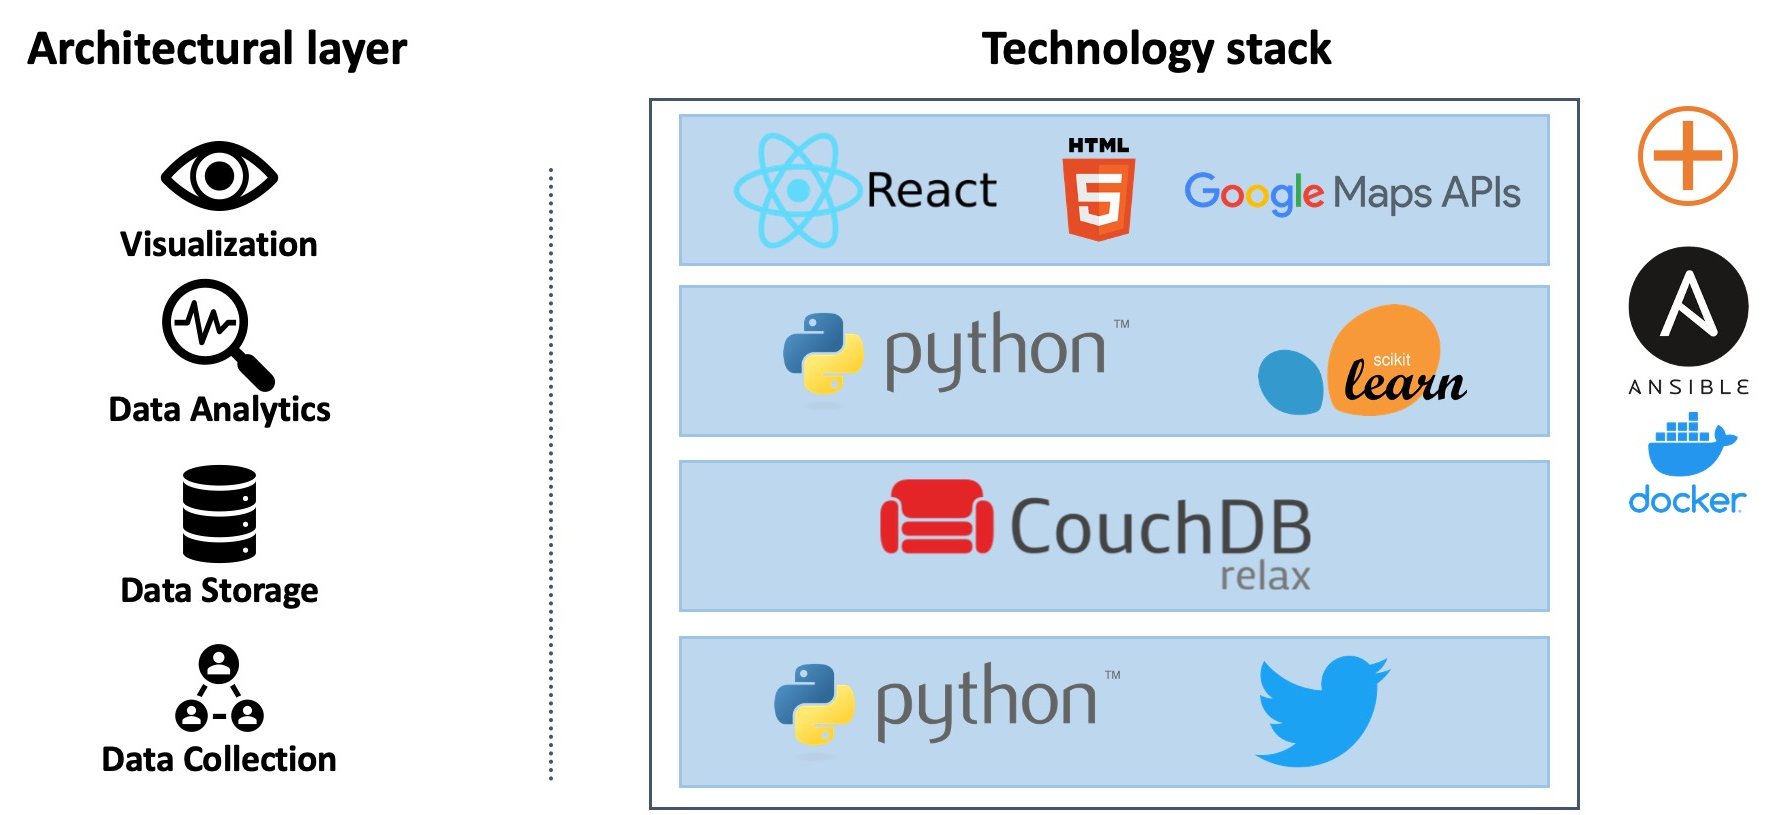
\includegraphics[width=0.8\linewidth]{figures/fig_system_design.png}  
\end{center}
  \caption{Reference architecture and core technology stack}
  \label{fig:system_design}
\end{figure}
The system architecture developed for this assignment was designed with a focus on scalability and reliability. It comprises a multi-layer architecture consisting of layer responsible for: 
\begin{myitemize}
    \item Data Collection
    \item Data Storage
    \item Data Analytics
    \item Data Visualization
\end{myitemize}
The architectural layers, as well as the respective technology stack (technologies and programming frameworks used for the assignment) are shown in figure \ref{fig:system_design} and are further described throughout this paper.

\subsection{General System Design}
% System design and architecture and how/why this was chosen
\begin{figure}
\begin{center}
      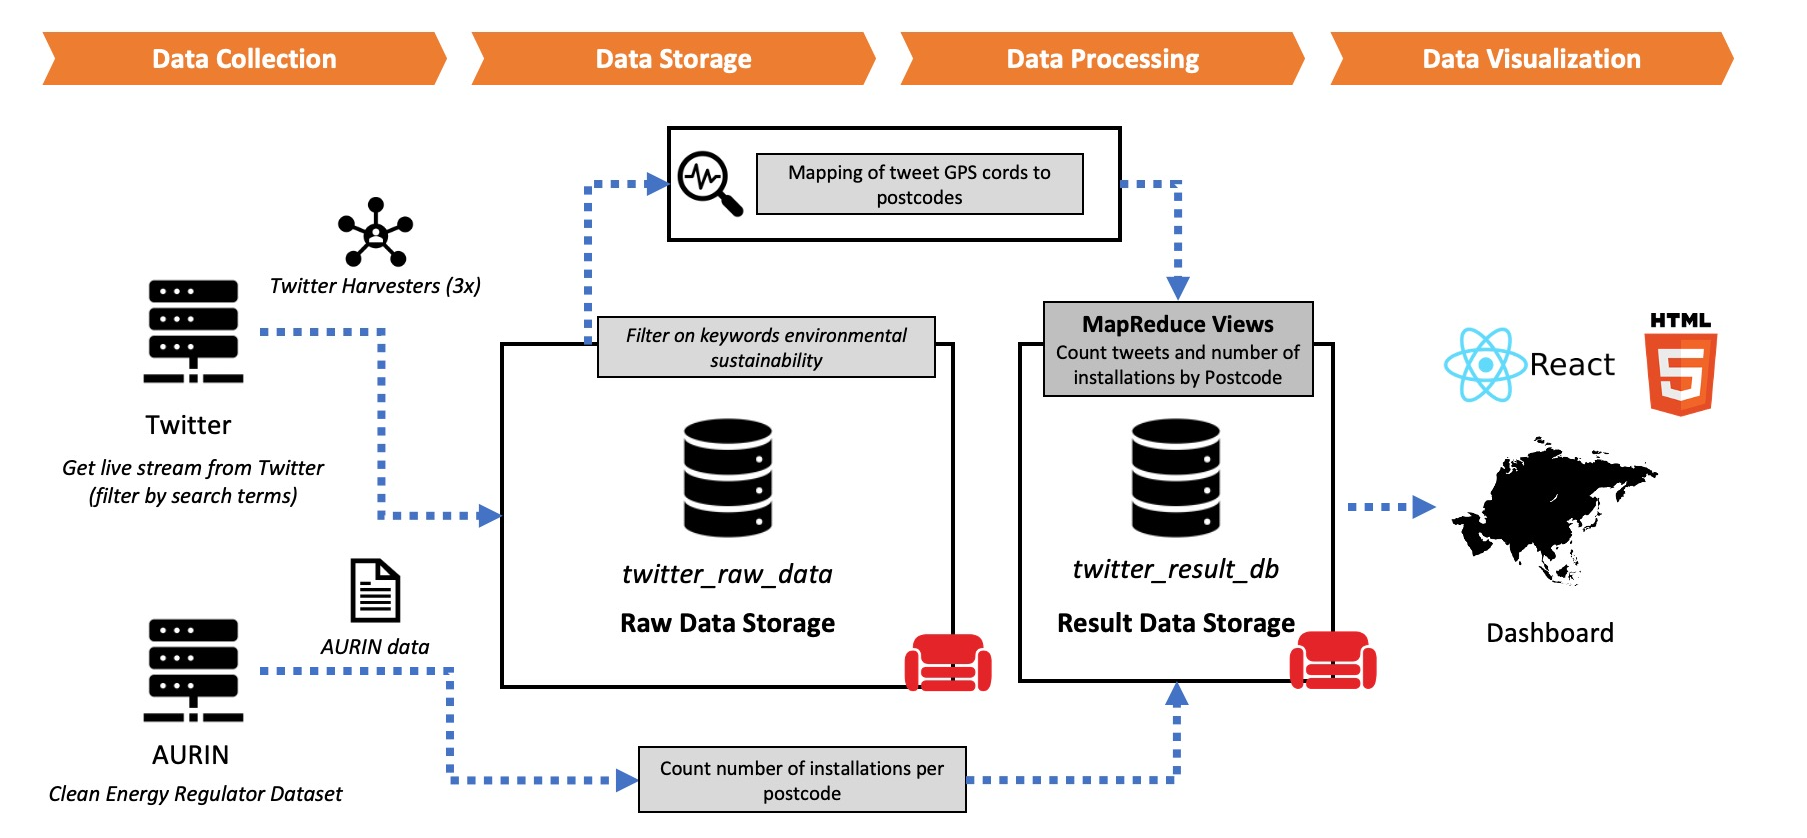
\includegraphics[width=0.8\linewidth]{figures/fig_data_pipeline.png}
\end{center}
  \caption{Data Pipeline}
  \label{fig:data_pipeline}
\end{figure}
Core focus of this assignment was to build up a data pipeline which is capable of handling data being streamed into the system in real-time. The data pipeline that was built for this purpose is shown in figure \ref{fig:data_pipeline}. It shows how data is being collected from various twitter harvesters and stored in a database called \textit{twitter\_raw\_data}. In order to analyze the collected tweet data and compare it with the \acrshort{cer} dataset extracted from \acrshort{aurin}, the GPS coordinates of each individual record first had to be converted to postcodes (as the dataset was only available on a postcode level). 
\newline
To accomplish this, a data processing component was created which extracts tweets from the raw data storage, processes it and stores the resulting information in a new database \textit{twitter\_result\_db}. This information is subsequently accessed and displayed in the web-based visualization frontend.

\subsection{System Deployment}
The whole system is deployed on a total of four computing instances running on the University of Melbourne Research Cloud. An overview of the computing nodes as well as their respective services is given in figure \ref{fig:system_deployment}.
\newline
Three of the four computing instances that were deployed on the cloud (\emph{server-01, server-02 and server-03}) have been designated as \enquote{Data Nodes}. Each Data Node runs an instance of the Twitter Harvester and the CouchDB database in a Docker container environment, thereby providing the opportunity for future scaling in case it is required.
\newline
\emph{Server-04} has been designated as the \enquote{Processing Node} which takes care of processing and analyzing the data. It also hosts the components that are required for the running the web-based visualization frontend. All components again are being run a Docker container environment.
\begin{figure}
  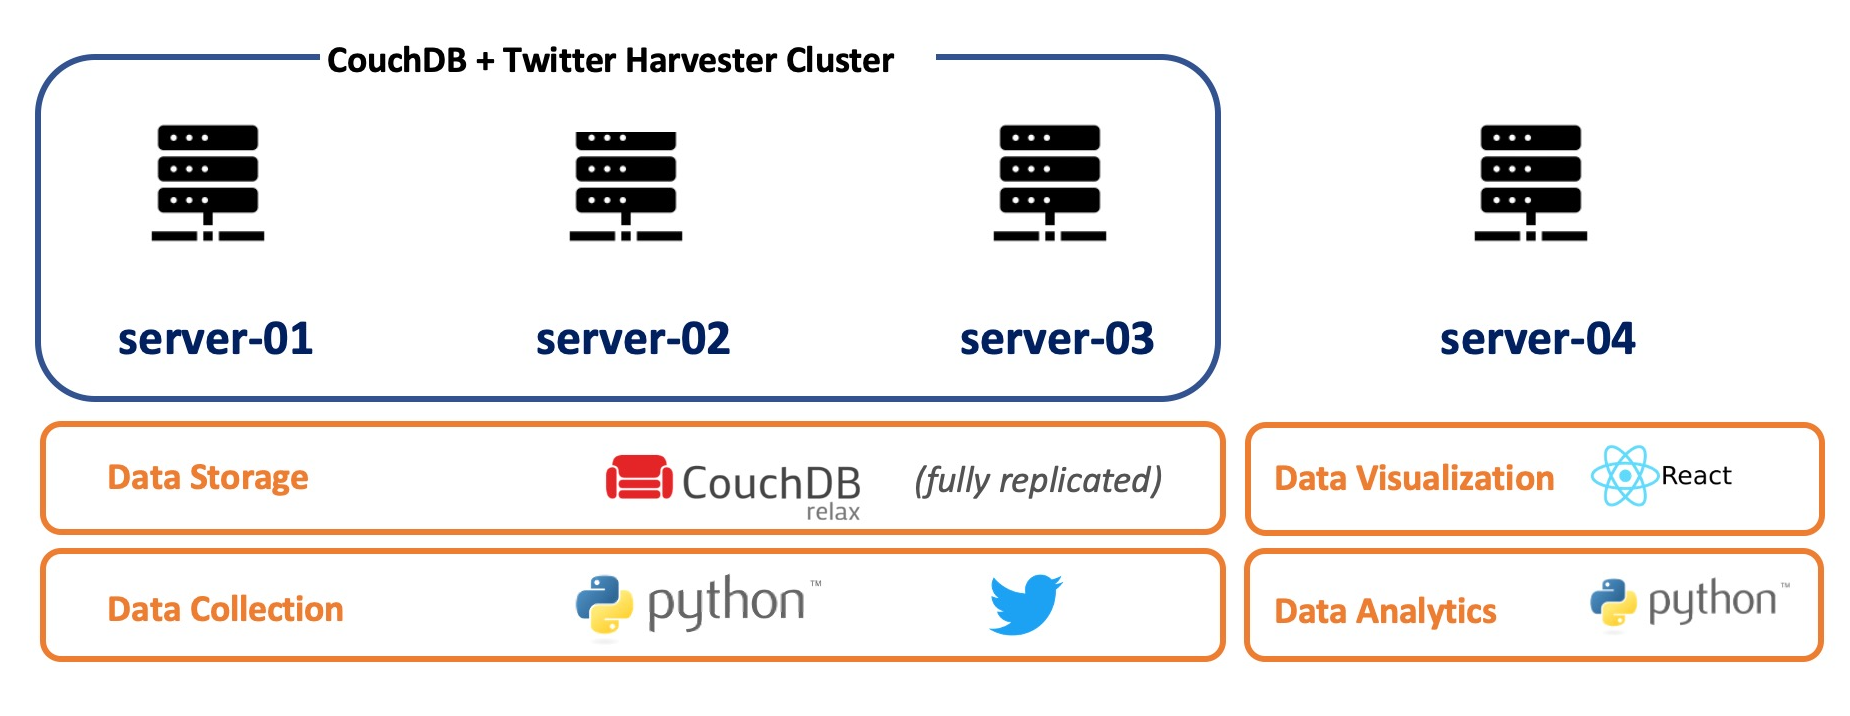
\includegraphics[width=\linewidth]{figures/fig_system_deployment.png}
  \caption{Reference architecture and core technology stack}
  \label{fig:system_deployment}
\end{figure}

\section{Cloud Infrastructure}
\label{sec:cloud_infrastructure}
The architecture described in this report makes use of the University of Melbourne Research Cloud infrastructure that was provided the course instructor. In addition to that, various cloud management and orchestration tools such as Ansible and Docker were used to facilitate the setup and deployment of the system architecture described in this assignment.

\subsection{Unimelb Research Cloud Infrastructure}
% discussion on the pros and cons of the UniMelb Research Cloud
The University of Melbourne operates its own cloud computing infrastructure which \enquote{comprises almost 20000 virtual cores, available across a range of instance sizes} \citep{unimelb_research_cloud}. The cloud infrastructure itself is built using the open-source implementation of OpenStack \citep{openstack} which allows the usage of existing libraries to access the OpenStack \acrfull{api}. 
\newline
Throughout the project and as a result of our continuous interaction with the University of Melbourne Research Cloud, various benefits and shortcomings were identified and are further listed below: 
\newline
\newline
\textbf{Benefits}
\begin{myitemize}
    \item \textit{Cross-cloud portability:} The deployment scripts and source code for this assignment are interoperable with any hosting provider that runs the OpenStack software, thereby limiting lock-in effects and allowing for future migration in case necessary 
    \item \textit{Usability:} The University of Melbourne Research Cloud provides a visually-appealing frontend interface via the OpenStack Horizon service as well as an \acrshort{api} to allow programmatic provisioning of new resources
\end{myitemize}

\textbf{Shortcomings}
\begin{myitemize}
    \item \textit{Limitations in available services:} Commercial public cloud offerings such as Amazon AWS or Microsoft Azure provide a vast amount of services which can be used to speed-up application development (e.g. DevOps integration etc.). In comparison to that, the OpenStack technology appears to be less mature.
    \item \textit{Limitations in available resources:} The resource allocation for the project did not allow the provisioning of computing instances with public (i.e. externally-accessible) IP addresses. The deployed infrastructure is therefore only available from within the University network, hence limiting its potential user base
\end{myitemize}

\subsection{Ansible Cloud Orchestration}
\begin{wrapfigure}{r}{0.3\textwidth}
  \begin{center}
    \fbox{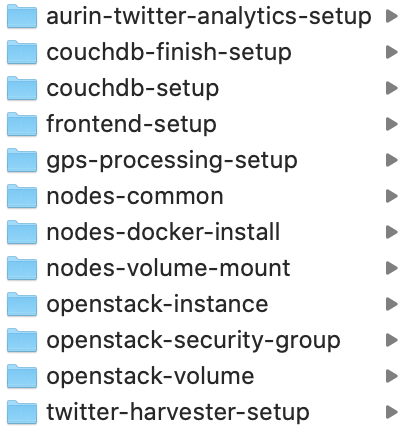
\includegraphics[width=0.3\textwidth]{figures/fig_ansible_playbook_tasks.png}}
  \end{center}
  \label{fig:ansible_playbook_tasks}
  \caption{Ansible Playbook Tasks}
\end{wrapfigure}
To enable dynamic scaling of the computing resources within the cloud environment, the Ansible technology stack was used for orchestration of all components within the system. Ansible enables its users to \enquote{scale automation, manage complex deployments and speed productivity with enterprise automation platform} \citep{ansible} and is therefore highly suited for this kind of tasks. 
\newline
The Ansible playbook that was created for this assignment enables the deployment and setup of the whole system from scratch (a process which is often referred to as \enquote{bootstrapping}). Overall, a total of twelve tasks are part of the playbook. The full overview of the Ansible playbook tasks that have been created for this assignment is presented in figure 4.
\newline
The tasks are responsible for executing the following steps:
\vspace{5pt}
\newline
\vspace{5pt}
\fcolorbox{black}{gray!15}{
\begin{minipage}{\columnwidth}
\textbf{Ansible Bootstrapping Steps}
\\[0.5cm]
\textbf{Step 1:} 
\newline
Provisioning of new cloud resources (computing instances, storage volumes, security groups) 
\newline
\textbf{Step 2:} 
\newline
Mounting and configuration of storage volumes on computing instances
\newline
\textbf{Step 3:} 
\newline
Installation of software packages (e.g. Python, Docker etc.)
\newline
\textbf{Step 4:} 
\newline
General configuration steps (e.g. configuration of proxy settings for Docker)
\newline
\textbf{Step 5:} 
\newline
Deployment and configuration of CouchDB and twitter harvester source code on DataNodes
\newline
\textbf{Step 6:} 
\newline
Deployment and configuration of data analytics scripts and web-based visualization frontend on Processing Node
\end{minipage}}
\newline
\newline
Ansible follows the \acrfull{iaac} paradignm which refers to the automatic management and deployment of computing infrastructure via machine-readable configuration files. This approach ensures repeatable and predictable deployments, while simultaneously reducing the need for interactive, tedious configuration steps. 


\subsection{Docker Container Technology}
The system implementation leverages a Microservice-based architecture using the Docker container technology for application deployment. Each service runs within its own container and exposes specific functionality to the applications that are interacting with it. 
\newline
Whenever a new service is deployed, an Ansible task is executed which clones the Git repository\footnote{Team 24 - Assignment 2 Git Repository: \url{https://github.com/Bachfischer/cluster-and-cloud-computing-assignment-2}} containing the application source code for this assignment. Each service has it's own directory within the repository which contains a Dockerfile. The Ansible task subsequently builds the Docker Container as instructed in the Dockerfile, stores the image inthe local repository of the node and executes the Docker image. 
\newline
This approach has allowed the authors of this paper to frequently deploy new increments of the individual services as more and more features were being implemented. In addition to that, having all the components that are required for the deployment of the system available in isolated Docker containers further facilitated local development work, as part of the system could be quickly set-up for testing and troubleshooting purposes.


\section{Data Collection}
\label{sec:data_collection}
This section describes the process that is involved in data collection. Section \ref{sec:twitter_data_harvesting} describes the setup that was used to harvest data from Twitter, while section \ref{sec:aurin_data_mining} describes the various ways in which data from \acrshort{aurin} was mined. Section \ref{sec:geojson_standard} further introduces the GeoJSON standard that was leveraged to display information on maps.

\subsection{Twitter Data Harvesting}
\label{sec:twitter_data_harvesting}
% In-order to harvest tweets from twitter, a script was written utilizing the Tweepy library \citep{tweepy} developed for Python.The harvester is highly scalable and dynamic in its design.In order to provide a light-touch way of being able to configure the harvesters dynamically and without having to redeploy them by changing application source, a tight integration with CouchDB was implemented.The harvesters work in a way that they dynamically fetch configuration parameters at a fixed interval (every one minute). This enables the authors of this paper to change config parameters, e.g. in order to adapt search terms\\
The Twitter harvester has been developed using the Python programming language. For the implementation, the authors have used the Tweepy library \citep{tweepy} to access the Twitter \acrshort{api} methods. The harvester has been developed as a dynamic and scalable solution with a tight integration into the  CouchDB storage environment. This allows to expand the scale of the harvester without needing to taking the system offline. 
\newline
This features of \enquote{zero-downtime update} is achieved by storing the Twitter \acrshort{api} credentials , the cities to scrape the tweets from and the search terms we are looking for in 3 databases  in the CouchDB setup, allowing us to expand  the number of credentials we have, number of cities we are searching in and the the search terms we are looking for in our targeted tweets on the fly. \\\\
\begin{figure}
  \begin{center}
  \fbox{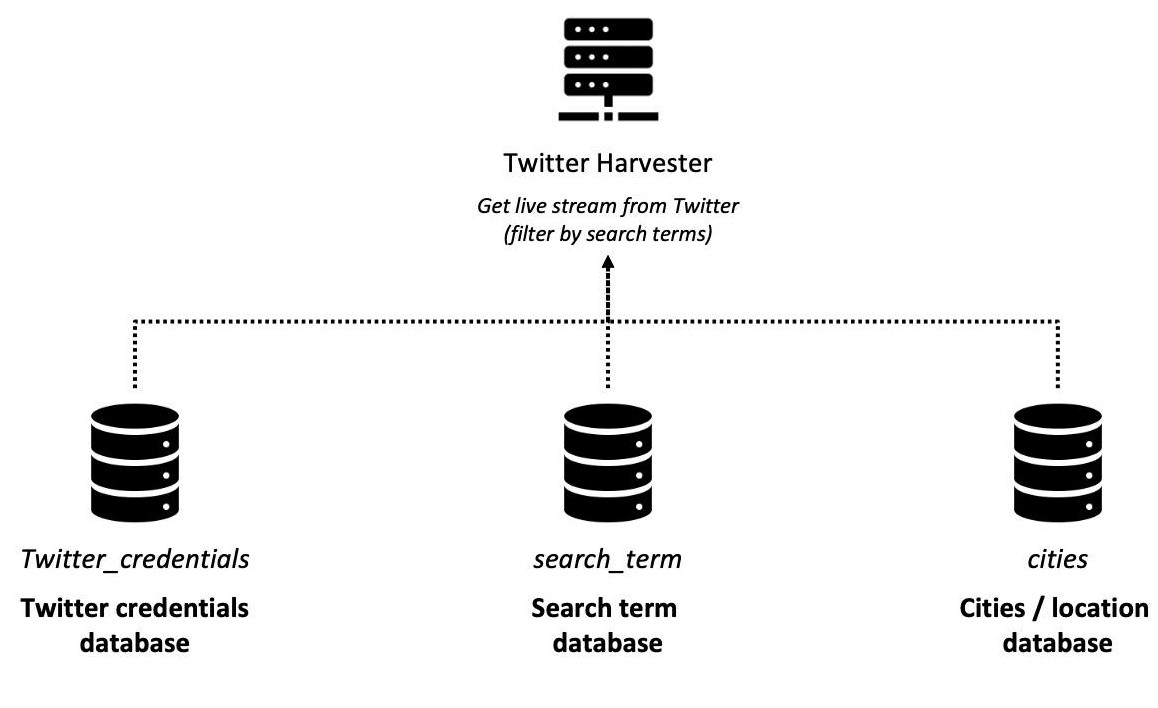
\includegraphics[width=0.8\linewidth]{figures/fig_twitter_harvester_database.jpg}}
  \end{center}
  \caption{Database support for Twitter Harvester}
  \label{fig:Database support for Twitter Harvester}
\end{figure}
The overall Harvesting process can be defined as the following:
\begin{enumerate}
    \item The harvester searches for an available Twitter \acrshort{api} credential (i.e. credentials which are not being used by any other harvester instance or whose rate limit has not been reached). If a valid set of credentials is found, it blocks the credentials using a flag so as to not allow any other harvester to access it concurrently. If no credentials are found , then the harvester goes to sleep.
    \item Similar to the Twitter \acrshort{api} credentials, the harvester looks for cities which are not being used for harvesting .
    \item Next, the harvester randomly searches for 20 key search terms from a list of search terms and constructs the search query.
    \item Through randomization, the harvester decides which configuration (the function arguments) of the search \acrshort{api} followed by the streaming \acrshort{api}.If a satisfactory tweet is found, it is stored in the database with the corresponding tweet ID as the record ID. However, before storing, a check is executed to see whether a record with the same ID already exists in the database or not. This way, it can be ensured that no duplicate data is stored.
    \item Whenever a Twitter \acrshort{api} error (e.g. in the form of rate limit) is reached or no more data is available, the harvester looks for the next set of available credentials and city and the whole process begins again.
\end{enumerate}
Besides the more generic functionality to harvest tweet data from Twitter at large-scale, the Tweet harvesting component of the system employs a variety of elaborate features to ensure robustness and ease-of-use. 
\newline
Some of the salient features are:
\begin{itemize}
    \item Usage of up to 10 twitter \acrshort{api} credentials from various accounts to ensure continuous data colelction when the rate limit is reached
    \item Ability to scan the present stream of tweets as well as to \enquote{go back in time} and search for missed out tweets using the \texttt{max\_id} and \texttt{since\_id} information in conjunction with the Twitter \acrshort{api}.
    \item Handling of the Twitter \acrshort{api} rate limit in two different ways:
    \begin{enumerate}
        \item Usage of multiple Twitter \acrshort{api} credentials so that if the rate limit is reached, another set of credentials is used
        \item Recording of the timestamp of the last usage of a particular Twitter credentials set (so that only credentials which were last used 15 minutes ago are being selected by the Twitter Harvester). 
    \end{enumerate}
\end{itemize}

\subsection{AURIN Data Mining}
\label{sec:aurin_data_mining}
This project used the \acrfull{ncris}-enabled \acrfull{aurin} Portal e-Infrastructure to access CER - Small-scale Installations - Solar Water Heater - Solar Panel (POA) on April 29th, 2020 \citep{sinnott2015australia}. This analysis was undertaken using the Spatialise Aggregated Dataset tool, implemented in the NCRIS-enabled Australian Urban Research Infrastructure Network (AURIN) Portal e-Infrastructure on April 29th, 2020. This tool was used to generate shape files for rendering the cities analyzed on the web app. 
\newline
\newline
The data used from \acrshort{aurin} was published by the \acrfull{cer} on a yearly basis. The \acrshort{cer} records the number of small scale renewable energy installations throughout Australia \citep{aurin_cer_dataset}. These installations are grouped based on postcodes, and the data is then filtered to contain only the postcodes within the \acrfull{gccsa} for each state, excluding Tasmania. The data that is used spans from the timeframe from 2001 to 2018.
\newline
\newline
The data set originally included installation numbers on a month-by-month basis, the total number of installations in a year, and the associated postcode, but the focus was on the total number of installations per year. After downloading this data from \acrshort{aurin}, it was then possible to loop through all of the years of the data and compile a new file that had the total number of installations from the entire 17 year period. These were then used as a measurement of the \enquote{action taken} by the people in that postcode. The data was stored via CouchDB and access it at any point we desired. 
\newline
\newline

\begin{figure}{H}
  \begin{center}
  \fbox{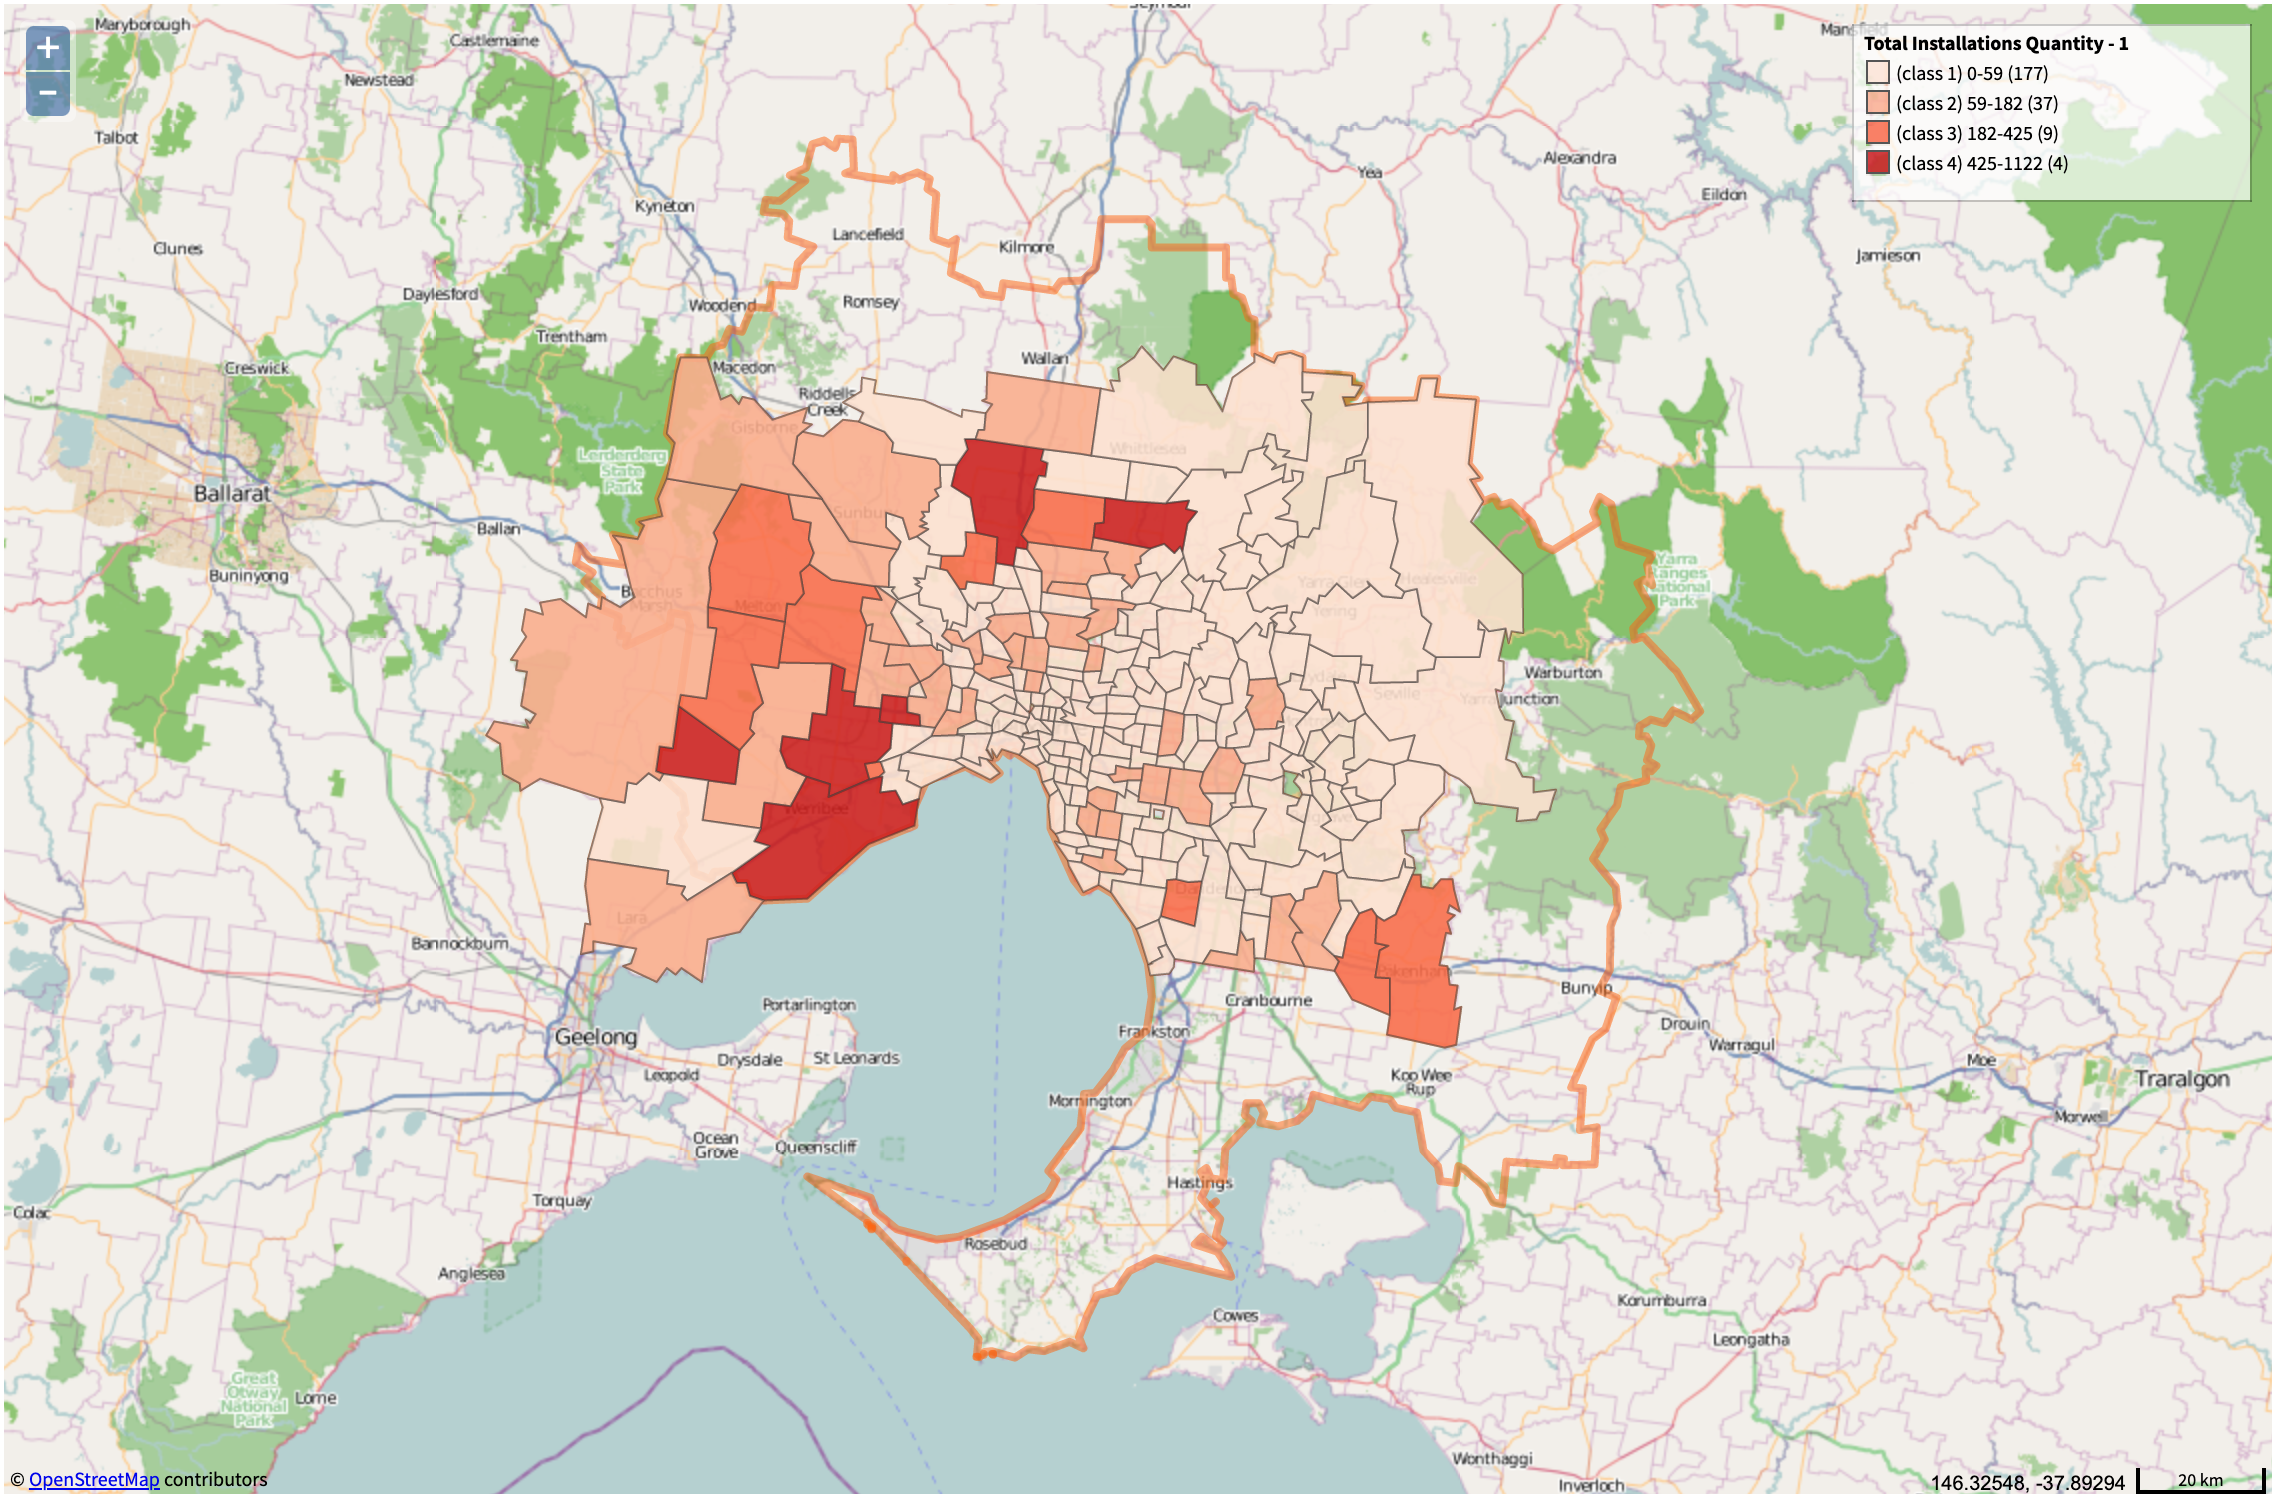
\includegraphics[width=0.8\linewidth]{figures/fig_aurin_choropleth.png}}
  \end{center}
  \caption{Distribution of installations around Melbourne installations}
  \label{fig:Distribution of installations around Melbourne}
\end{figure}

The other data extracted from Aurin were the shape files that were associated with the installation data. Using the spatialise dataset tool, it was then possible to generate shape files for every postcode. These shape files were then used to extracted the GeoJSONs within them. Once the GeoJSONs were extracted, it was run through the external tool Mapshaper \citep{mapshaper} to reduce the granularity of the boundaries. This reduction in boundary detail also led to a reduced file size. After extracting the necessary GeoJSONs, the day was stored in a database with the associated total installations.
\newline
\newline
After looking at the more granular data grouped by postcodes, we then decided to also look at the data based on the \acrshort{gccsa} as a whole, instead of their respective postcodes. To do this, we retrieved the Aurin data we stored via CouchDB that was the summation of installations in all of the postcodes within GCCSAs spanning 2001-2018. We then looped through all of the different postcodes within these GCCSAs and summed up all of the total installations per year. This resulted in the total number of installations in each \acrshort{gccsa} over the course of the 17 year period. 
\newline
\newline
Through initial data exploration, it was observed that installations were usually clustered around the outer parts of the GCCSAs, as this is where there were likely new homes being built and new buildings being developed. This can be seen in Figure 5, which is a choropleth map of the Melbourne area.

\subsection{GeoJSON Standard}
\label{sec:geojson_standard}
The GeoJSON standard follows the the format specified in RFC 7946 \citep{rfc7946} stating that \enquote{GeoJSON is a geospatial data interchange format based on the JavaScript Object Notation Language (JSON)}. The sections of RFC 7946 that were of most interest for this project were that of section 3.1.6 and 3.1.7 which are that of the polygon and multipolygon. These follow certain rules allowing for their standardised use in APIs such as the Maps JavaScript API\footnote{Maps Javascript API reference:\url{https://developers.google.com/maps/documentation/javascript/reference}}
\newline
\newline
For example, a city may comprise of multiple polygons to make up the area that the city encompasses with potentially many different 'holes' for natural features such as lakes where information may be irrelevant. Suburbs, being relatively small in comparison, tend to have just a polygon feature in the GeoJSON but can still contain the 'holes' as mentioned above.
\newline
\newline
The fact that GeoJSON follows the standards of a standard \acrshort{json} meant that very little manipulation had to be performed to ensure communication between the components was standardised.

\section{Data Storage}
\label{sec:data_storage}
The data storage layer for this system was built using the CouchDB database technology. Three nodes (\emph{server-01, server-02 and server-03}) were chosen to form a CouchDB database cluster described in \ref{sec:CouchDB_database_cluster}. Various components of the system rely on CouchDB for storage and persistence - they are shown in section \ref{sec:overview_databases}. 

\subsection{CouchDB Cluster Setup}
\label{sec:CouchDB_database_cluster}
CouchDB is a flexible, modern NoSQL database which can be tailored for a variety of use cases. It can furthermore be configured for operation in a clustered environment in order to \enquote{improve on the single-node setup with higher capacity and high-availability} \citep{couchdb}. 
\newline
For this assignment, the readily-available Docker images provided by IBM\footnote{CouchDB 3.0 Docker Image published by IBM: \url{https://hub.docker.com/r/ibmcom/CouchDB3}} were used, as those particular images already include a variety of features suchas as the Clouseau CouchDB text index plugin. Following this, two Ansible tasks \textit{CouchDB-setup} and \textit{CouchDB-finish-setup} were created which are responsible for installing and configuring the CouchDB Docker containers.
\newline
The configuration parameters and credentials that are needed for the setup of the CouchDB cluster are stored as variables within the respective Ansible tasks and are passed to the installer during install time.
\newline
In order to enable the operation CouchDB in a clustered mode, various prerequisites need to be fulfilled: The security groups used by the computing instances need to be adjusted to allow inter-node communication on \acrfull{tcp} port 4369, 5984 and port range 9100 - 9200, a consistent \acrfull{uuid} needs to be set and default credentials for access to the database need to be defined.

\subsection{Database Overview}
\label{sec:overview_databases}
The CouchDB database is an integral part of various components of the system architecture at hand and is responsible for
\begin{enumerate}
    \item Storage of raw and processed tweets that were collected from Twitter 
    \item Storage of configuration parameters for Twitter Harvesters (e.g. Twitter \acrshort{api} credentials, Target GPS coordinates of Australia's cities
    \item Storage of processed \acrshort{aurin} data for comparison in scenario analysis
\end{enumerate}
An overview of the databases that were used for this assignment is provided in figure \ref{fig:CouchDB_database_overview}. Of particular importance is the database \textit{twitter\_raw\_data} which holds the \enquote{raw} tweets that were collected by harvesting the twitter \acrshort{api}, as well as the database \textit{twitter\_result\_db} which holds the tweets after they have been processed and allows aggregation of the data on a per-postcode level.
\begin{figure}
  \begin{center}
  \fbox{\includegraphics[width=0.8\linewidth]{figures/fig_CouchDB_database_overview.png}}
  \end{center}
  \caption{Overview of CouchDB databases used as part of this project}
  \label{fig:CouchDB_database_overview}
\end{figure}

\section{Data Processing}
\label{sec:data_processing}
The system involves two major kinds to data processing. Section \ref{sec:gps_to_postcode_processing} describes the step which are required to convert GPS coordinates in tweets to postcodes, while section \ref{sec:mapreduce_analytics} further elaborates how the system leveraged CouchDBs built-in MapReduce analytics capabilities. In addition to that, various experiments involving advanced analytics were performed - they are described in section \ref{sec:advanced_data_analytics}.

\subsection{GPS to Postcode Processing}
\label{sec:gps_to_postcode_processing}
The conversion of GPS coordinates to postcodes involves the process of taking each record from the \enquote{raw} database \textit{twitter\_raw\_data}, extracting the geo-locations present in these records (i.e. the latitude and longitude from where the Tweet was initially posted) and converting it to an address. From the address we obtain the postcode information and we use that to perform detailed regional analysis of the tweets. 
\newline
\newline
Data processing is achieved with the help of a python script which runs continuously to get all the records from the database which have geo-locations and are not yet converted to postcode. In the case that all the records have been converted the script waits for a minute and then keeps re-checking the database for newer Tweets. This process continues throughout the lifetime of the project.
\newline
\newline
For the implementation of the GPS conversion, the Python library Geopy \citep{geopy} was used. This library provides a python client for several popular geocoding web-services which allow the conversion the latitude and longitude information to an address from which we obtain the postcode information. This information is subsequently updated with the rest of the data in the record to the \enquote{result} database \textit{twitter\_result\_db} where it is stored eventually for further analysis with the \acrshort{aurin} data.
\newline
\newline
Only those latitudes and longitudes which return a postcode are stored in the Result database while the others are left out. Some of the tweets are \enquote{geo-enabled} which means that their latitude and longitude information are highly accurate as their users have attached their current location to their tweets. The tweets that are \enquote{geo-enabled} are differentiated from the tweets that are only available on a per-city level in the frontend visualization. 

\subsection{MapReduce Analytics}
\label{sec:mapreduce_analytics}
MapReduce was used to count the amount of tweets that occurred at each postcode. Since many tweets lacked precise GPS information, the postcodes were further aggregated into self-defined, \enquote{city-wide postcode} with a dummy value of the city's central business district postcode + 10,000 (i.e. the postcode that reflects all tweets within Melbourne area is 3000 + 10,000 = 13,000) . 
\newline 
This approach allowed the system to count GPS-enabled data separately to the data which was only available on a per-city level and did not have location data. This not only made it easier both to count but also to display on the website. 
\newline
MapReduce was further implemented using the view function given by CouchDB where '\_count' was the reduce used.
\subsection{Advanced Data Analytics}
\label{sec:advanced_data_analytics}
Besides the processing of tweet information in real-time within the system, a variety of additional, additional advanced analytics techniques were applied in order to generate a better understanding of the contents of the data set and verify initial hypotheses. 
\begin{figure}
    \centering
    \begin{subfigure}[b]{0.3\textwidth}
        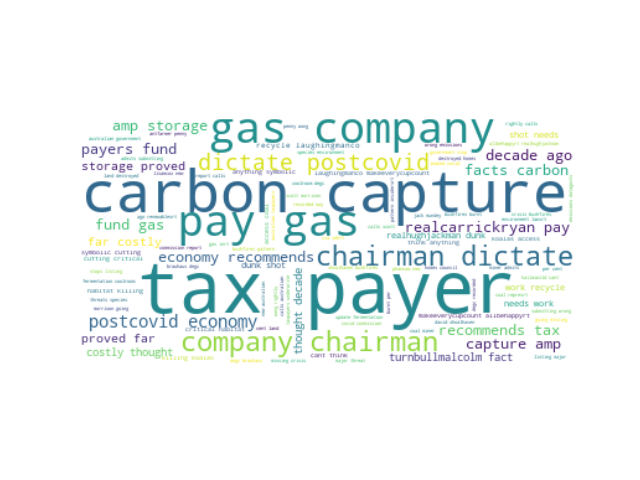
\includegraphics[width=\textwidth]{figures/sydney_word_cloud.png}
        \caption{Sydney}
    \end{subfigure}
    ~ %add desired spacing between images, e. g. ~, \quad, \qquad, \hfill etc. 
      %(or a blank line to force the subfigure onto a new line)
    \begin{subfigure}[b]{0.3\textwidth}
        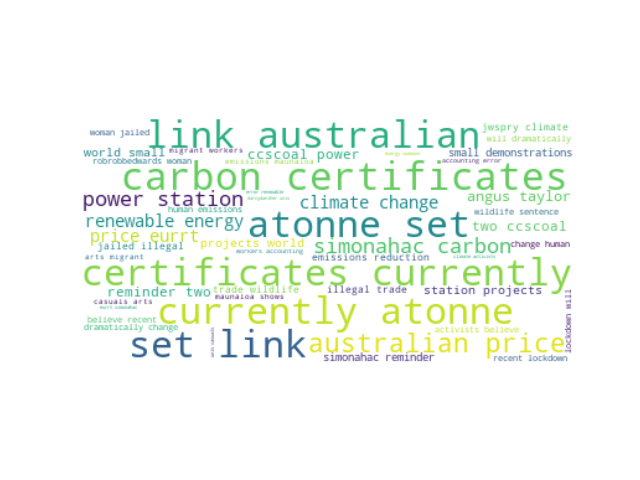
\includegraphics[width=\textwidth]{figures/melbourne_word_cloud.png}
        \caption{Melbourne}
    \end{subfigure}
    ~ %add desired spacing between images, e. g. ~, \quad, \qquad, \hfill etc. 
    %(or a blank line to force the subfigure onto a new line)
    \begin{subfigure}[b]{0.3\textwidth}
        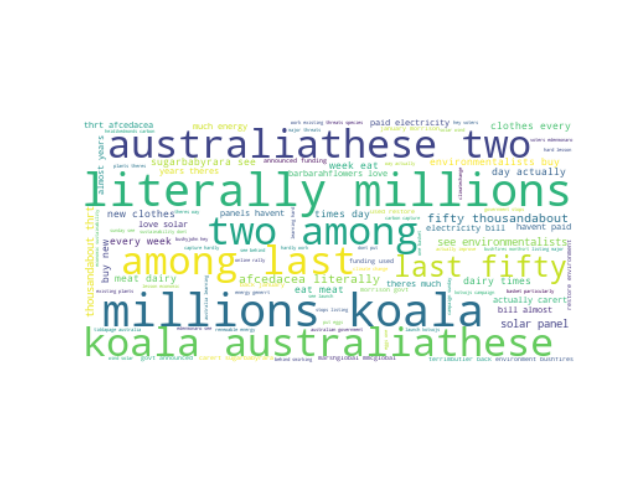
\includegraphics[width=\textwidth]{figures/perth_word_cloud.png}
        \caption{Perth}
    \end{subfigure}
    \caption{Word clouds for cities in Australia}
    \label{fig:word_clouds}
\end{figure}
\newline
Amongst others, two of the approaches that were used for his kind of advanced data analytics are:
\begin{enumerate}
    \item Generation of word clouds (i.e. most commonly mentioned words)
    \item Calculation of polarization and subjectivity scores on a per-city level
\end{enumerate}
By generating word clouds, the authors of this paper wanted to create a visually-appealing representation of the most commonly mentioned words in tweets. An example of the word clouds that were generated for Sydney, Melbourne and Perth is shown in figure \ref{fig:word_clouds}.
\newline
\newline
Since environmental sustainability is generally regarded as a highly controversial topic, the authors of this paper were interested in better understanding the sentiment of Australians when tweeting about that topic. Figure \ref{fig:sentiment} shows polarization scores for the cities of Melbourne, Sydney and Adelaide.
\newline
The polarization scores are calculated using a Python library called TextBlob which returns a float value between -1 and 1 where -1 indicates highly negative statement while 1 indicates positive statement .
\begin{figure}[h!]
    \centering
    \begin{subfigure}[b]{0.3\textwidth}
        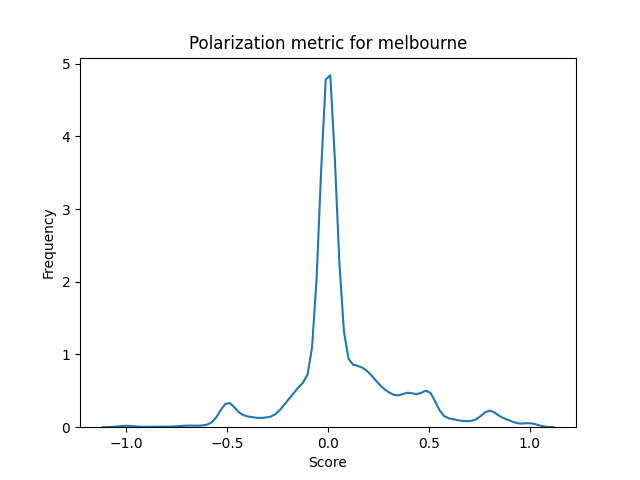
\includegraphics[width=\textwidth]{figures/polarization_melbourne.png}
        \caption{Melbourne}
    \end{subfigure}
    ~ %add desired spacing between images, e. g. ~, \quad, \qquad, \hfill etc. 
      %(or a blank line to force the subfigure onto a new line)
    \begin{subfigure}[b]{0.3\textwidth}
        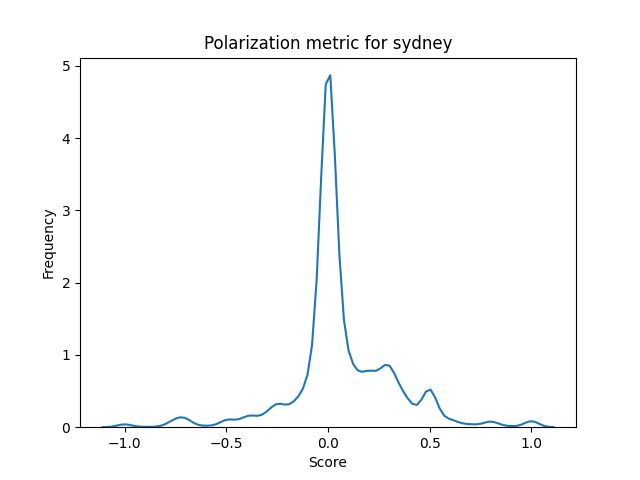
\includegraphics[width=\textwidth]{figures/polarization_sydney.png}
        \caption{Sydney}
    \end{subfigure}
    ~ %add desired spacing between images, e. g. ~, \quad, \qquad, \hfill etc. 
    %(or a blank line to force the subfigure onto a new line)
    \begin{subfigure}[b]{0.3\textwidth}
        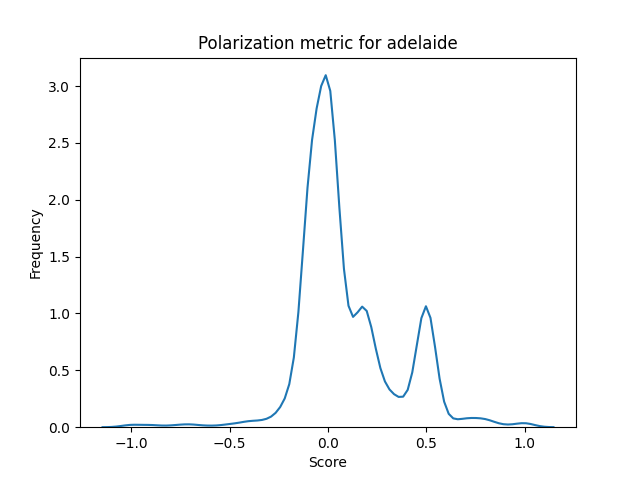
\includegraphics[width=\textwidth]{figures/polarization_adelaide.png}
        \caption{Adelaide}
    \end{subfigure}
    \caption{Polarization scores for cities in Australia}
    \label{fig:sentiment}
\end{figure}
\newline

\section{Data Visualization}
\label{sec:web_frontend}
This section describes the Frontend data visualization component that was implemented for this assignment. It consists of a backend data caching component described in section \ref{sec:backend_data_caching} as well as a frontend data visualization component presented in section \ref{sec:frontend_data_visualization}.

\subsection{Backend Data Interface}
\label{sec:backend_data_caching}
The back-end consists of a Node.js application that facilitates the retrieval of information from CouchDB. It provides a \acrfull{rest} \acrshort{api} the enables the frontend to easily retrieve specific sets of data from the database (e.g. tweet statistics per city). 
\newline
\newline
The relevant information to be displayed is found in separate databases. The database \texttt{geo\_json} contains pre-processed AURIN data which is separated into suburbs stored as GeoJSONs, while the database \texttt{twitter\_result\_db} contains the accumulated and processed tweets. These needed to be joined so that the information could be easily gathered from the back-end and passed on to be visualised by the front end. The script uses MapReduce functionality (as discussed above) to gather the count of the tweets from each postcode and join them with the appropriate GeoJSON where it was stored in the properties section where it maintains the standards for the use of a GeoJSON. 
\newline
From the tweet count and the AURIN data which can be found in the properties, the ratio between the installations of solar panels and the tweet count of a suburb are calculated and stored in the GeoJSON. This reduces the need to do advanced processing on the frontend. This final GeoJSON is subsequently stored in the database \texttt{postcode\_aurin}' within CouchDB where it could be retrieved.
\newline
\newline
The back-end does not perform any processing on the data. It is rather used as a way to retrieve data from the database when queried by the front-end. A JavaScript package called nano \citep{nano} facilitates the access of CouchDB with the use of views such as the retrieval of all suburbs or cities. This is done through the provided CouchDB \acrshort{rest} \acrshort{api}. 
\newline
\newline
When attempting to retrieve data from the database, the backend will query a URL that contains the appropriate view which was created on CouchDB. This view provides the frontend with the data is has requested. A similar process occurs during communication betweenthe frontend and the backend. It queries a URL that resolves to a certain route on the backend where the process of receiving information from the database is implemented..

\subsection{Frontend Data Visualization}
\label{sec:frontend_data_visualization}
The front end is built in JavaScript using the web framework React. This technology stack was chosen as it provided easy access to libraries that facilitated the use of google maps as a means to present the data. This data has been displayed using the shape files acquired from AURIN. 
\newline
\newline
The front end queries the backend dependent on what the page attempted to display. The home page shows the distinction between the different capital cities of each state and therefore only requires the retrieval of the GeoJSON on a per-city level. Google maps is then rendered once the file has been retrieved with the focus being initially on the main areas surveyed on a city wide level, Melbourne, Canberra, Sydney and Adelaide. 
\newline
\newline
Information on specific, geo-enabled tweet locations was low and so the use of suburb information has been relegated to a secondary page where individual cities are rendered on google maps. This also allows for better comparison between the local ratios of each suburb against one another. 
\newline
\newline
Polygons are the main method for displaying the shapes on the Google Maps API. The GeoJSON data provides this in the form of polygons as well as multi-polygons which were handled separately but rendered in the same way. As these polygons had their sizes reduced the act of retrieving and displaying them was greatly reduced form the original files.
\newline
\newline
A white to red scale was used to represent the ratio of each suburb. The more red the suburb was, the higher the ratio. These ratios are shifted from their original range to a distribution between 0 and 255 allowing the conversion to hexadecimal and therefore an RGB colour grade scaling form white to red.
\newline
\newline
A table underneath describes the total tweets and installations per city or postcode, if you are on the suburbs page, where it shows the ratio received by the front end of each area that has been seen. 


\section{User Guide}
\label{sec:user_guide}

The source code for this assignment is available online under the following repository \acrshort{url}: 
\newline
\newline
\textbf{Source Code Repository:}
\newline
\url{https://github.com/Bachfischer/cluster-and-cloud-computing-assignment-2}.
\newline
\newline
\textbf{Demonstration of Web App:}
\newline
\url{http://172.26.130.40}.
\newline
\newline
\textbf{Video Demonstration:}
\newline
\url{https://youtu.be/7oCPjouVqUs}.
\newline
\newline
It contains all relevant application code as well as the Ansible playbook that is required to deploy and setup the system from scratch.

\subsection{System Deployment}
To deploy (i.e. bootstrap) the  system from scratch, first make sure that you have Ansible installed and available on your machine. Next, clone the source code repository and navigate to the \emph{deployment} directory within the repository. 
\newline
Execute the \emph{run\_bootstrap\_infrastructure.sh} script in a Linux shell. The script will ask you for your OpenStack API password, and after entering the password, the Ansible playbook which is defined in \emph{bootstrap\_infrastructure.yaml} will be executed and deployed.

\subsection{Usage of visualization frontend}
Shown below is the main page that a user is greeted with when entering the site. The ratio is displayed at the bottom of the map indicating which colours show the highest and lowest of the cities displayed on the map (figure \ref{fig:cities_visualization}).
\newline
\newline
\begin{figure}
  \begin{center}
  \fbox{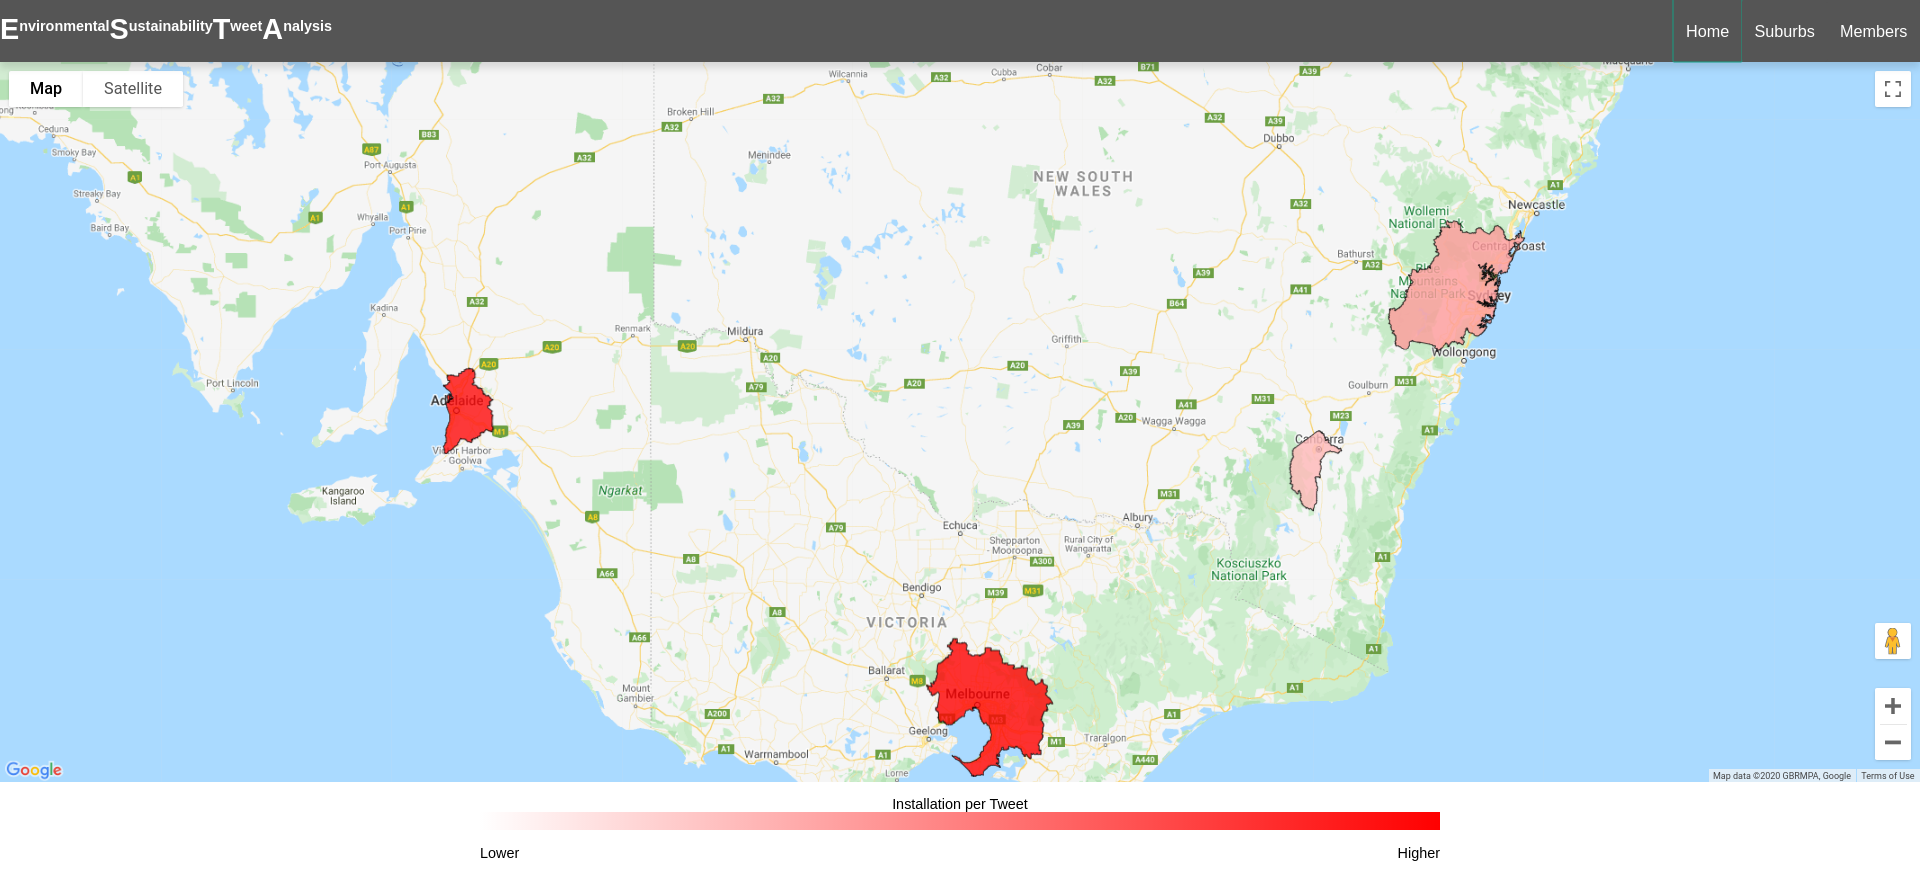
\includegraphics[width=0.8\linewidth]{figures/fig_cities.png}}
  \end{center}
  \caption{Home page, displaying a ratio comparison between cities}
  \label{fig:cities_visualization}
\end{figure}
The user can then click the suburbs button up the top left where it will take them to the secondary page (figure \ref{fig:melbourne_suburbs_visualization}). This shows the user user the ratio of installations per tweet of each suburb in a particular city. The starting city is Melbourne. From there the user can click on one of the 4 other cities that they may wish to check up on. 
\newline
\newline
\begin{figure}
  \begin{center}
  \fbox{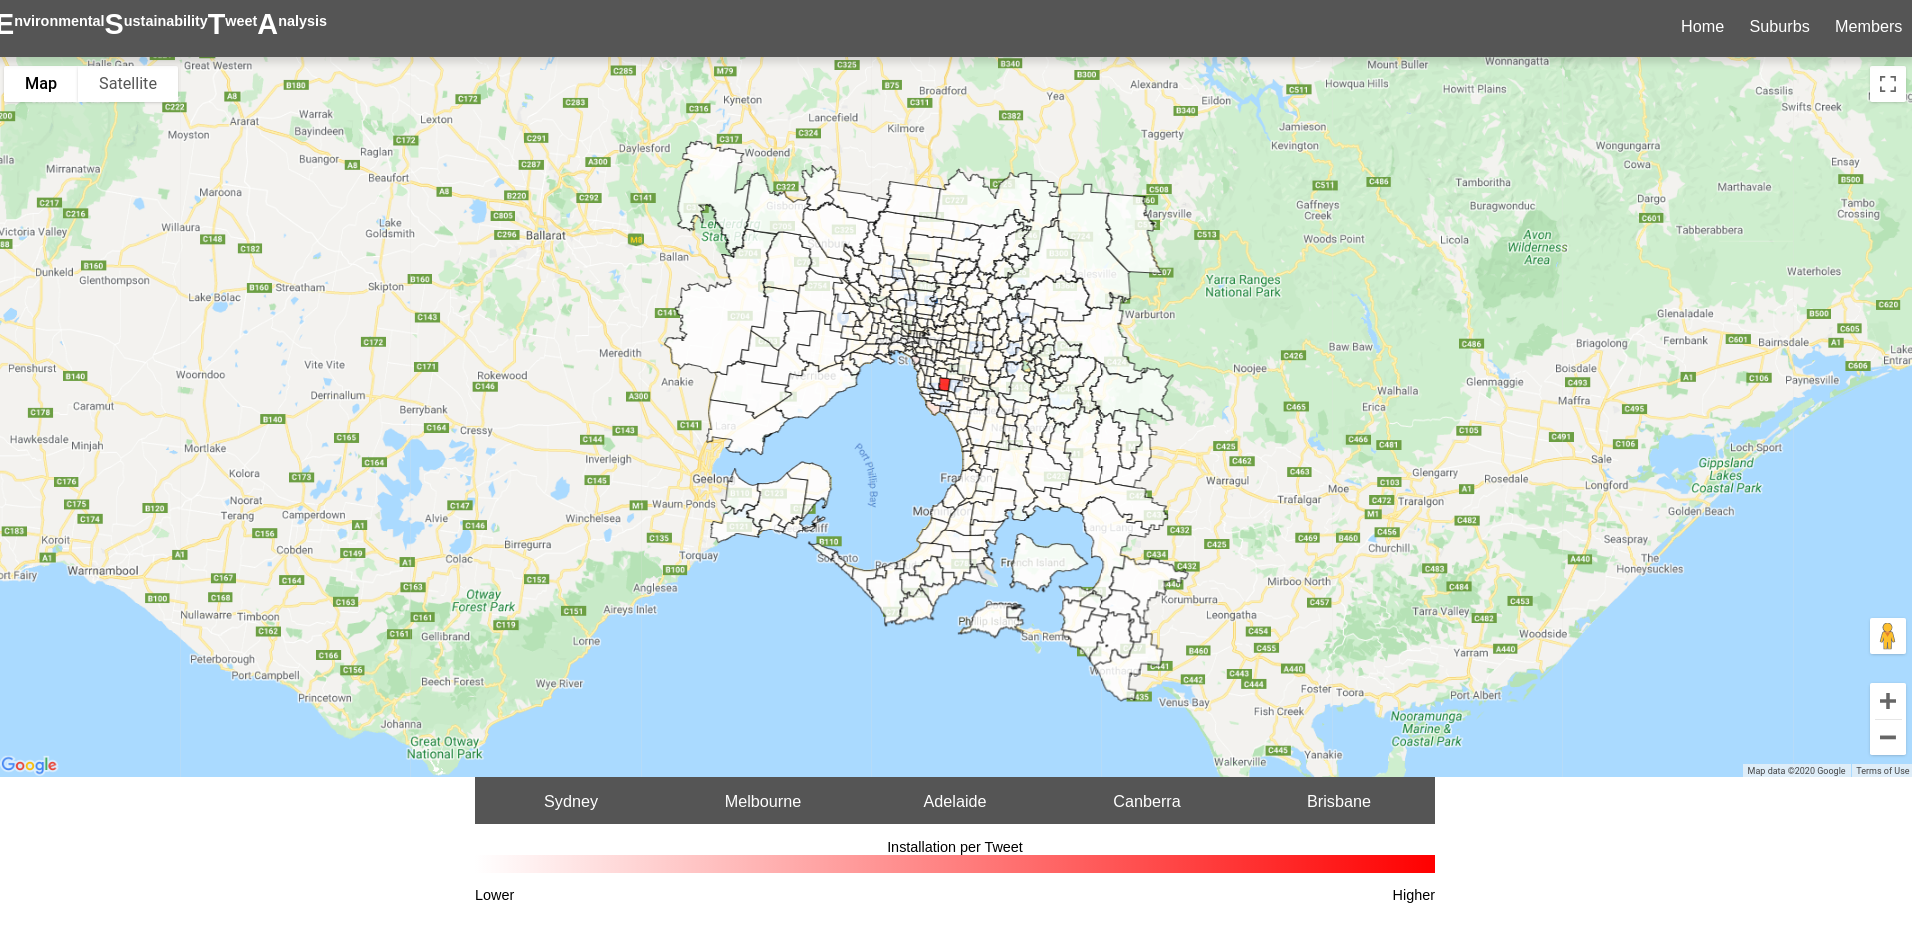
\includegraphics[width=0.8\linewidth]{figures/fig_suburbs.png}}
  \end{center}
  \caption{Suburb Page, displaying a ratio comparison between city suburbs}
  \label{fig:melbourne_suburbs_visualization}
\end{figure}
An example of this is the user clicking Adelaide below the map where they will be taken to the vicinity of Adelaide as seen in figure \ref{fig:adelaide_suburbs_visualization}.
\newline
\newline
\begin{figure}
  \begin{center}
  \fbox{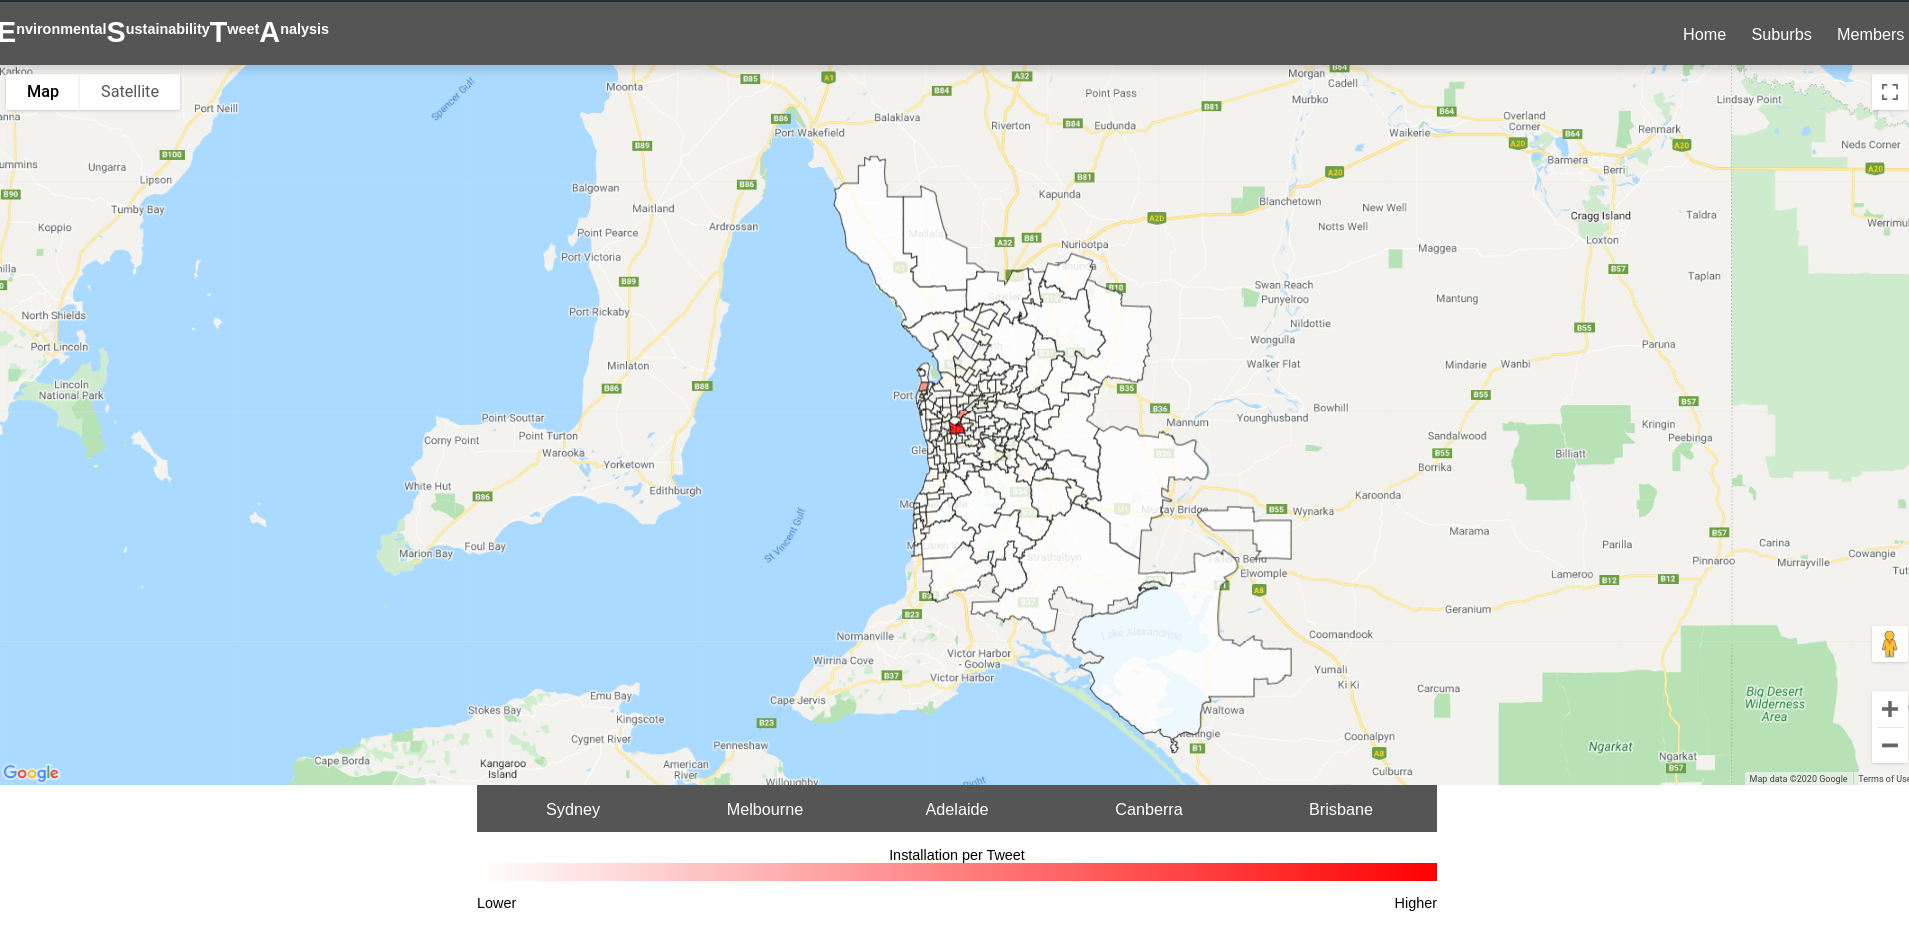
\includegraphics[width=0.8\linewidth]{figures/fig_suburbs_adelaide.png}}
  \end{center}
  \caption{Changing cities will display that cities ratio comparison}
  \label{fig:adelaide_suburbs_visualization}
\end{figure}
Under each of the maps the user can find a table displaying the relevant information for the city or cities that they are viewing. For example when visiting the map on the front page then the table displayed is that of all the cities and when visiting a specific city on the suburb page the table that will be displayed is that of the suburbs in the city that have at least one tweet (figure \ref{fig:suburb_table}).
\newline
\newline
\begin{figure}
  \begin{center}
  \fbox{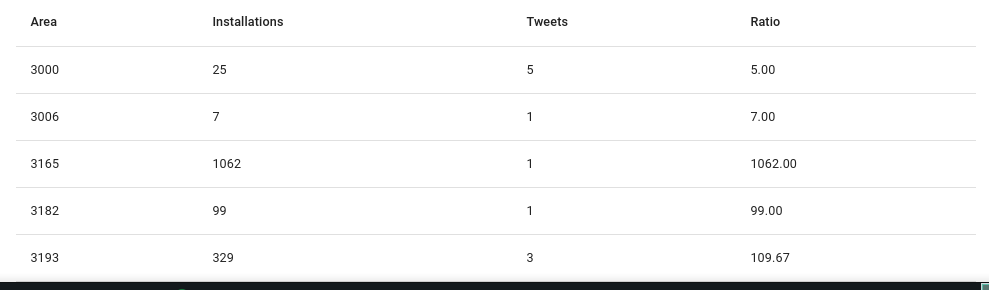
\includegraphics[width=0.8\linewidth]{figures/fig_table_suburbs.png}}
  \end{center}
  \caption{Table of information on suburbs with a tweet count}
  \label{fig:suburb_table}
\end{figure}

\section{Team Collaboration}
\label{sec:team_collaboration}
The assignment was delivered by working and collaborating as a highly-integrated, cross-functional team. Each of the team members was tasked with a separate set of responsibilities which are further stated in table 1. The core programming language for this assignment was Python, as all members of the team were familiar with that programming language. 
\newline
Throughout the implementation period, a variety of digital tools such as Zoom\footnote{Zoom Video Conference Software: \url{https://zoom.us}} (virtual meetings) or Trello\footnote{Trello Project Management Tool \url{https://trello.com/b/mjCUm91f/cluster-and-cloud-computing}} (task tracking) were leveraged. 
\begin{table}
\resizebox{\textwidth}{!}{%
\begin{tabular}{ll}
\hline
\textbf{Team member} & \textbf{Responsibilities}                                                                          \\ \hline
Liam Simon           & \begin{tabular}[t]{@{}l@{}} - Implementation of web-based visualization frontend\\ - Implementation of middleware and connection to backend\\ - MapReduce of Tweet information and attachment to AURIN data through scripting\end{tabular}                         \\[1.1cm]
Colin McLean         & \begin{tabular}[t]{@{}l@{}}  - Downloading data from Aurin\\ - Feature engineering with AURIN data \\ - Assistance with Twitter harvesters and analzying tweet data \end{tabular}                 
\\[1.1cm]
Parikshit Diwan      & \begin{tabular}[t]{@{}l@{}}- Implementation of highly-scalable Twitter harvester setup\\ - Analyzing Twitter data to generate insights among cities \end{tabular}                  
\\[1.1cm]
Matthias Bachfischer & \begin{tabular}[t]{@{}l@{}}- Deployment of cloud infrastructure \\ - Setup of CouchDB\\ - Orchestration of applications\end{tabular} 
\\[1.1cm]
Rejoy Benjamin       & \begin{tabular}[t]{@{}l@{}} - Generic data processing scripts\\ - Conversion of GPS coordinates to postcodes\end{tabular}                                 
\\[0.7cm]
\hline
\end{tabular}%
}
\label{tab:team_responsibilities}
\caption{Overview of team responsibilities}
\end{table}


\section{Conclusion}
\label{sec:conclusion}
The observed results were expected for some cities and more surprising for others. The measure of \enquote{taking actions} to rhetoric was taken by the ratio of installations per tweet. The results can be observed in figure \ref{fig:ratio_tweet_activity_solar_panels}. The highest ratio of installations to tweets is in the greater Adelaide area, followed by Sydney, Melbourne, and lastly Canberra. The top two \acrlong{gccsa} are both over ten, while the bottom two \acrlong{gccsa} are five and under. 
\newline
\newline
Population size and the size of the \acrlong{gccsa}s are important to take into consideration when looking at the results. Melbourne and Sydney both have populations hovering around 5 million, while Adelaide has 1.3 million, and Canberra has 300,000 people. Sydney has the largest area in terms of square kilometers, but is still comparable to Melbourne. Adelaide and Canberra have a considerably smaller area in terms of square kilometers, so one would expect to see less installations and less tweets in these two areas. 
\newline
\newline
The inner city suburbs of Melbourne have had elected officials who are a part of the Green Party. Therefore, it makes sense that they also have the highest number of installations. However, Melbourne also has the highest amount of tweets relating to climate change. Because their installations were so much higher than the other areas, their ratio was still the top. This shows that people in Melbourne care about creating a sustainable future, and they are also acting on their words.
\begin{figure}
  \begin{center}
  \fbox{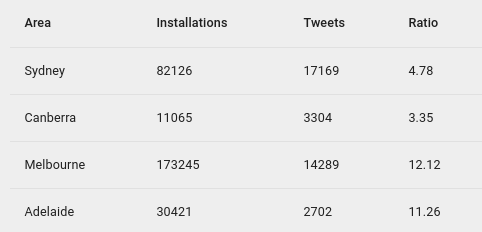
\includegraphics[width=0.8\linewidth]{figures/fig_city_ratios_chart.png}}
  \end{center}
  \caption{Ratio of tweet activitiy and solar panel installations}
  \label{fig:ratio_tweet_activity_solar_panels}
\end{figure}
Sydney has the second most installations in the analyzed areas. Similarly to Melbourne, they also have a high number of tweets. They have a high number of installations due to the high amount of squared kilometers in the \acrlong{gccsa}, and a high number of tweets due to the large population size. Their low ratio shows that although people in Sydney are talking about climate change and they care about these issues, they are not necessarily taking action to create a more sustainable future.
\newline
\newline
Adelaide has the second highest ratio of installations per tweet. This means that there are many people acting on their words. Also note that Adelaide has the lowest number of people tweeting about issues related to climate change. An explanation for these results could be the fact that Adelaide has the oldest median age of the four areas that were analyzed \citep{age_statistics}. It is expected that those who are older also tweet less. In addition to this, Adelaide has a smaller population size than Sydney and Melbourne.
\newline
\newline
Canberra has a reputation of being a \enquote{green} city, and the average income is high due to the bureaucratic nature of the capital city. There are a plethora of well paying jobs, so those who live in this \acrlong{gccsa} have the means to install solar panels if they so desire. However, we can see that Canberra has the lowest ratio of the four analyzed cities. It is worth noting that the Canberra area is also the smallest size in terms of square kilometers, so there is less space to be installing these solar panels.
\newpage


\printbibliography[heading=bibintoc]


\end{document}
